\section{采样模型}
\label{sec:mrec-sampling}

要讨论“由样本恢复流形”，先要说清样本与流形是什么关系，以及用什么尺度衡量“足够密”“足够近”“足够平”。本章始终固定一个紧致、无边界的光滑嵌入子流形$M\subseteq\mathbb R^D$，维数为$m$，它可以有有限个连通分支。先讨论样本恰好落在$M$上的情形，再单独加入离开流形的扰动。

有三种容易混淆的距离。环境距离$\lVert\bm x-\bm y\rVert_2$是$\mathbb R^D$中的直线距离，任意两点都能算。内在距离$d_M(\bm p,\bm q)$是第~\ref{chap:riemannian-geometry}章在嵌入诱导度量下定义的距离，只对$M$上的点有意义；两点在不同分支时约定为$+\infty$。样本间距则是样本彼此相隔多远，是样本自身的属性。

打个比方，环境距离是打穿地球的直线隧道，内在距离是沿地表走的路程。两点靠得很近时二者几乎相同，隔得远时可以相差很多。本章的很多论证，都是在“小尺度上二者接近”这一点上做文章。

本节引入的覆盖精度和可达半径是对$M$与样本关系的假设，用来陈述“在什么条件下恢复成立”。它们不能从有限样本中准确读出：只看样本，无法知道流形在两个样本之间是否藏着一个小褶皱。

\subsection{样本覆盖}
\label{sec:mrec-coverage}

样本能否代表流形，首先要看流形上有没有远离所有样本的地方。设$P=\{\bm p_1,\ldots,\bm p_n\}\subseteq M$是有限样本。

\begin{definition}[稠密样本]
\label{def:mrec-dense-sample}
设$\delta>0$。若对每个$\bm x\in M$都存在$\bm p\in P$使$\lVert\bm x-\bm p\rVert_2<\delta$，则称$P$是$M$的$\delta$\term{稠密样本}（dense sample）。
\end{definition}

把每个样本换成半径$\delta$的开球，定义说的就是这些球盖住了整个$M$。函数$\bm x\mapsto\min_{\bm p\in P}\lVert\bm x-\bm p\rVert_2$在紧集$M$上连续，所以有最大值，记为
\begin{equation}
 \delta_P=\max_{\bm x\in M}\ \min_{\bm p\in P}\lVert\bm x-\bm p\rVert_2 ,
 \label{eq:mrec-covering-radius}
\end{equation}
称为$P$的覆盖精度。它是流形上最孤立的那一点到最近样本的距离，$P$是$\delta$稠密样本当且仅当$\delta_P<\delta$。图~\ref{fig:mrec-coverage}(a)画的是一条闭曲线和覆盖它的小圆盘。

单位圆上取$n$个等距样本，可以直接算出覆盖精度。最孤立的点是相邻两样本之间的弧中点，它到最近样本的圆心角是$\pi/n$，对应的弦长就是
\[
 \delta_P=2\sin\frac{\pi}{2n}.
\]
于是$n=6$时$\delta_P=2\sin15^\circ\approx0.518$，$n=24$时$\delta_P=2\sin3.75^\circ\approx0.131$。这两组数后面会反复用到。

定义用的是环境距离。同一对点的环境距离不超过内在距离，所以内在意义下稠密蕴含环境意义下稠密；反过来不一定，因为环境中靠近的两点沿流形可能很远。

\begin{BookInlineFigure}
  \centering
  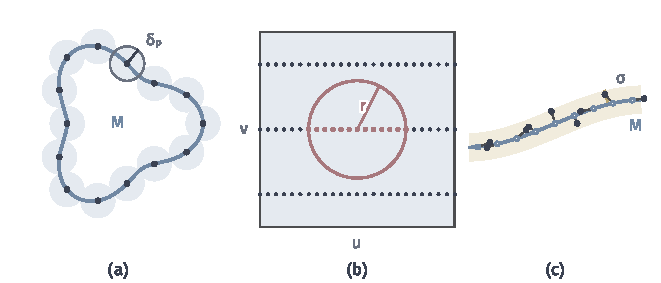
\includegraphics[width=112mm]{figures/04-spaces-measures-and-geometry/04-manifolds/matplotlib/mrec-coverage/figure.pdf}
  \caption{样本与流形的三种关系。(a) 曲线上$14$个样本（黑点），半径取覆盖精度$\delta_P$的圆盘把曲线盖满。(b) 一块平坦区域上的三条水平样本线，全域稠密，但红圈内的样本全在一条线上，只提供$u$方向的信息。(c) 观测（黑点）由真实采样点（空心点）沿任意方向偏移不超过$\sigma$，都落在曲线的$\sigma$管状邻域（浅黄）内。}
  \label{fig:mrec-coverage}
\end{BookInlineFigure}

\paragraph{局部邻域}

后面的局部计算都在某个位置附近进行。对选定的中心$\bm c\in\mathbb R^D$和半径$r>0$，记邻域样本为
\begin{equation}
 N_r(\bm c)=\{\bm p\in P:\lVert\bm p-\bm c\rVert_2\leq r\}.
 \label{eq:mrec-neighborhood}
\end{equation}
中心可以是一个样本，也可以是需要估计的任意位置。选邻域有定半径和定点数两种做法。本章采用定半径，因为$r$是一个明确的几何尺度，可以直接与覆盖精度和后面的可达半径比较；按点数选取时，各处的半径随采样疏密而变。

\paragraph{全域稠密与方向分布}

全域稠密只说明每一点附近都有样本，并不说明在某个邻域内，样本沿流形的各个方向都铺开了。设$M$的一块区域是平的，用坐标$(u,v)\in[0,1]^2$表示，例如平环面上的一小块。在这块区域上只沿三条水平线$v=\tfrac16,\tfrac12,\tfrac56$取样，每条线上的样本间距为$\tfrac1{24}$，如图~\ref{fig:mrec-coverage}(b)。

这组样本在全域上相当密。最孤立的点在两条水平线的正中间，又在两个相邻样本的正中间，所以
\[
 \delta_P=\sqrt{\bigl(\tfrac16\bigr)^2+\bigl(\tfrac1{48}\bigr)^2}\approx0.168 .
\]

现在以水平线上的一个样本为中心取半径$r=0.25$。相邻水平线的间隔是$\tfrac13>r$，所以邻域里的$13$个样本全在同一条水平线上。它们沿$u$方向铺开，完全不提供$v$方向的信息，后面的局部线性拟合会得到秩不足的矩阵。

所以全域稠密不能单独保证局部拟合的秩和条件数，邻域内的方向分布要另作要求。第~\ref{sec:mrec-tangent-error}节把这一要求写成局部矩阵的特征值条件。

\subsection{观测扰动}
\label{sec:mrec-noise}

实际观测很少恰好落在流形上。把第$i$个观测写成
\begin{equation}
 \bm x_i=\bm p_i+\bm e_i,\qquad\bm p_i\in M,\quad\lVert\bm e_i\rVert_2\leq\sigma ,
 \label{eq:mrec-noise-model}
\end{equation}
其中$\bm p_i$是看不到的真实采样位置，$\bm e_i$是环境空间中的有界扰动，方向任意，如图~\ref{fig:mrec-coverage}(c)。

这一模型把两种误差分开记录：真实采样点的覆盖精度$\delta_P$描述流形上有没有空缺，扰动界$\sigma$描述观测离开流形多远。由三角不等式，每个观测到$M$的距离不超过$\sigma$；而$M$上任一点先走到最近的真实采样点，再走到对应的观测，所以
\[
 \min_i\lVert\bm x-\bm x_i\rVert_2\leq\delta_P+\sigma,\qquad\bm x\in M.
\]

扰动改变了能够谈论的对象。$\bm x_i\notin M$时，$\bm x_i$处的切空间没有定义，$d_M(\bm x_i,\bm x_j)$也没有定义，能估计的只是附近真实位置处的量。所以无噪声的结论不能直接搬过来，每个结论都要重新说明$\sigma$进入哪里。

不同的任务对$\sigma$的要求也不同。邻域选择只受环境距离影响，每个成对距离至多变化$2\sigma$。局部拟合要求$\sigma$相对邻域半径小，才能把法向噪声与沿流形的展开区分开。拓扑恢复要求$\sigma$相对流形本身的尺度小，否则噪声可能填掉细小的孔洞。后面各节分别处理。

本章把扰动看成确定的有界量，只问“给定这些界，结论是否成立”。若样本按某个分布随机抽取、噪声是随机变量，则覆盖精度与扰动界都变成随机量，要估计它们以多大概率不超过给定值，可参考\BookChapterRef{chap:finite-sample-error-bounds}{卷八第4章“有限样本的误差上界”}。

\subsection{可达半径}
\label{sec:mrec-reach}

覆盖精度只说明样本多密，还缺一个描述流形自身形状的尺度：样本要密到什么程度，才算“相对于流形足够密”？直观上，流形弯得越厉害，或者它的不同部分靠得越近，所需的样本就越密。这两种情况可以用同一个量刻画。

对$\bm x\in\mathbb R^D$，记$\bm x$到$M$的距离为
\[
 \operatorname{dist}(\bm x,M)=\min_{\bm p\in M}\lVert\bm x-\bm p\rVert_2 .
\]
由$M$紧致，最小值可以取到，取到最小值的点称为$\bm x$在$M$上的最近点。$M$上的点的最近点是它自己；离开$M$以后，最近点可能不唯一，例如平面上单位圆的圆心到圆上每一点的距离都是$1$。

把$M$向外加粗，记
\[
 M^r=\{\bm x\in\mathbb R^D:\operatorname{dist}(\bm x,M)<r\}.
\]
可以想象从$M$出发同时向四面八方“长肉”，$M^r$是长到厚度$r$时的形状。厚度很小时，$M^r$里的每一点都能找回唯一的出发点；厚度增大，从不同地方长出来的部分迟早相撞，相撞处的点就有了两个最近点。可达半径就是这个相撞发生之前的最大厚度。

\begin{definition}[可达半径]
\label{def:mrec-reach}
$M$的\term{可达半径}（reach）定义为
\begin{equation}
 \tau=\sup\{r\geq0:M^r\text{中每一点在}M\text{上都有唯一最近点}\}.
 \label{eq:mrec-reach}
\end{equation}
\end{definition}

半径为$R$的圆的可达半径为$R$：圆心以外的每一点都有唯一最近点，即沿径向的那一点，而圆心离圆的距离恰为$R$。对紧致无边界的光滑嵌入子流形总有$\tau>0$，这是管状邻域定理的推论，证明可查阅Federer关于曲率测度的论文。

在$M^\tau$内，可以定义最近点投影$\pi$：$\pi(\bm x)$是$\bm x$在$M$上唯一的最近点。这个投影是连续的。设$\bm x_k\to\bm x$都在$M^\tau$中，由$M$紧致，$\pi(\bm x_k)$的任一收敛子列有极限$\bm z\in M$，并且
\[
 \lVert\bm x-\bm z\rVert_2=\lim_k\lVert\bm x_k-\pi(\bm x_k)\rVert_2=\lim_k\operatorname{dist}(\bm x_k,M)=\operatorname{dist}(\bm x,M).
\]
所以$\bm z$是$\bm x$的最近点，由唯一性$\bm z=\pi(\bm x)$。每个收敛子列的极限都是$\pi(\bm x)$，于是$\pi(\bm x_k)\to\pi(\bm x)$。

最近点还有一条一阶条件：$\bm x-\pi(\bm x)$与$M$在$\pi(\bm x)$处的切空间垂直。这是因为沿$M$上过$\pi(\bm x)$的任一曲线，到$\bm x$的距离平方在$\pi(\bm x)$处取最小值，导数为零。

\paragraph{限制可达半径的三种情形}

可达半径同时受三种因素限制，图~\ref{fig:mrec-reach-limits}分别画出了它们。

第一种是局部弯曲。图中是长半轴$2$、短半轴$1$的椭圆。在长轴端点$(2,0)$处曲率半径为$b^2/a=\tfrac12$，沿内法向走到曲率中心$(\tfrac32,0)$，这里是所有“最近点不唯一”的位置组成的线段的端点。一般地，曲线上曲率为$\kappa$的点使$\tau\leq1/\kappa$，圆的情形正是$\tau=R=1/\kappa$，椭圆的可达半径正是$\tfrac12$。

第二种是同一分支的不同部分相互接近。图~\ref{fig:mrec-reach-limits}(b)的闭曲线在中部收窄，两股相距$2b$，那里的曲率并不大，但中点$\bm z$到上下两股的距离相等，有两个最近点，所以$\tau\leq b$。第三种是不同分支相互接近，这时分支之间的距离直接控制可达半径。

\begin{BookInlineFigure}
  \centering
  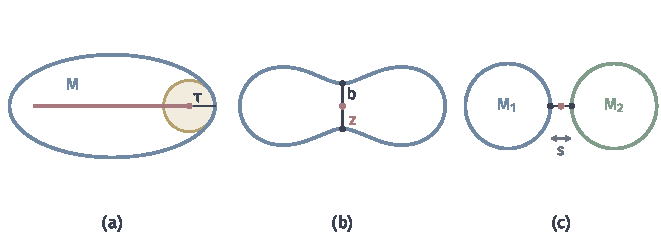
\includegraphics[width=112mm]{figures/04-spaces-measures-and-geometry/04-manifolds/matplotlib/mrec-reach-limits/figure.pdf}
  \caption{限制可达半径的三种情形。(a) 椭圆内部红色线段上的点都有两个或更多最近点，线段端点是长轴端点的曲率中心，到曲线的距离$\tau=\tfrac12$是这一位置的曲率半径。(b) 曲线中部收窄，中点$\bm{z}$有上下两个最近点，$\tau\leq b$。(c) 两个分支相距$s$，中点（红）同样有两个最近点，$\tau\leq s/2$。}
  \label{fig:mrec-reach-limits}
\end{BookInlineFigure}

\begin{lemma}[不同分支的间隔]
\label{lem:mrec-component-gap}
$M$的任意两个不同连通分支之间的环境距离不小于$2\tau$。
\end{lemma}
\begin{proof}
紧致流形只有有限个分支，每个分支紧致。所以在所有“属于不同分支”的点对中，环境距离的最小值$s$可以由某对$\bm p\in M_1$、$\bm q\in M_2$取到。

假设$s<2\tau$，取中点$\bm z=\tfrac12(\bm p+\bm q)$，则$\operatorname{dist}(\bm z,M)\leq s/2<\tau$，$\bm z$有唯一最近点$\bm w$。若$\lVert\bm z-\bm w\rVert_2=s/2$，则$\bm p,\bm q$都是$\bm z$的最近点，与唯一性矛盾，所以
\[
 \lVert\bm z-\bm w\rVert_2<\frac s2 .
\]

由三角不等式，
\[
 \lVert\bm p-\bm w\rVert_2\leq\lVert\bm p-\bm z\rVert_2+\lVert\bm z-\bm w\rVert_2<s,
\]
同样$\lVert\bm q-\bm w\rVert_2<s$。而$\bm w$所在的分支至少与$M_1$、$M_2$之一不同，这就找到了一对距离小于$s$的不同分支的点，与$s$的最小性矛盾。所以$s\geq2\tau$。
\end{proof}

\paragraph{可达半径控制的局部几何}

后面要用可达半径控制两件事：流形离切平面有多远，沿流形的路程比直线长多少。先看一个几何事实。在$\bm q\in M$处取单位法向量$\bm v$，沿它走一小段距离$s$，到达的点$\bm q+s\bm v$的最近点应当还是$\bm q$。下面的引理说，这一点一直保持到$s=\tau$。

\begin{lemma}[法向线段]
\label{lem:mrec-normal-segment}
设$\bm q\in M$，$\bm v$是$M$在$\bm q$处的单位法向量，$0\leq s<\tau$，则$\pi(\bm q+s\bm v)=\bm q$。
\end{lemma}
\begin{proof}
记$M$的法丛为
\[
 N=\{(\bm a,\bm w):\bm a\in M,\ \bm w\perp T_{\bm a}M\}.
\]
用局部的法向标准正交标架作坐标，可知$N$是$D$维流形。定义映射
\[
 \Phi:M^\tau\to N,\qquad\Phi(\bm x)=\bigl(\pi(\bm x),\ \bm x-\pi(\bm x)\bigr).
\]
由最近点的一阶条件，$\Phi$确实落在$N$中；由$\pi$连续，$\Phi$连续。

$\Phi$是单射，因为由$\Phi(\bm x)$相加两个分量就得到$\bm x$。$M^\tau$是$\mathbb R^D$的开集，$N$是$D$维流形，由Brouwer的区域不变性定理，连续单射$\Phi$的像$\Phi(M^\tau)$是$N$的开集。

令$A=\{s\in[0,\tau):\pi(\bm q+s\bm v)=\bm q\}$。首先$0\in A$。由$\pi$连续，$A$在$[0,\tau)$中是闭的。

再看$A$是开的。设$s\in A$，则
\[
 (\bm q,s\bm v)=\Phi(\bm q+s\bm v)\in\Phi(M^\tau).
\]
$\Phi(M^\tau)$是开集，所以当$s'$靠近$s$时$(\bm q,s'\bm v)$也在其中，即存在$\bm y\in M^\tau$使
\[
 \Phi(\bm y)=(\bm q,s'\bm v).
\]
相加两个分量得$\bm y=\bm q+s'\bm v$，并且$\pi(\bm y)=\bm q$，这就是$s'\in A$。

$[0,\tau)$连通，$A$既开又闭且非空，所以$A=[0,\tau)$。
\end{proof}

这条引理有一幅很直观的图像：在$\bm q$处沿法向放一个半径略小于$\tau$的球，球心是$\bm q+s\bm v$，引理说球内部不含$M$的点。可以想象一个半径为$\tau$的球沿$M$滚动，它能贴着$M$走遍每一点而不被挤开，如图~\ref{fig:mrec-rolling-ball}(a)。把这幅图写成不等式，就得到流形偏离切平面的界。

\begin{lemma}[法向偏离]
\label{lem:mrec-normal-distance}
对任意$\bm p,\bm q\in M$，$\bm q-\bm p$到切空间$T_{\bm p}M$的距离满足
\begin{equation}
 \operatorname{dist}(\bm q-\bm p,\ T_{\bm p}M)\leq\frac{\lVert\bm q-\bm p\rVert_2^2}{2\tau}.
 \label{eq:mrec-reach-normal}
\end{equation}
\end{lemma}
\begin{proof}
把$\bm q-\bm p$分解为切向部分与法向部分$\bm n$，式~\eqref{eq:mrec-reach-normal}的左端就是$\lVert\bm n\rVert_2$。$\bm n=\bm 0$时不用证，否则令$\bm v=\bm n/\lVert\bm n\rVert_2$。

对$0<s<\tau$，由引理~\ref{lem:mrec-normal-segment}，$\bm p$是$\bm p+s\bm v$的最近点，所以$\bm q$到它的距离不小于$s$：
\[
 \lVert\bm q-\bm p-s\bm v\rVert_2^2\geq s^2 .
\]
展开左端，并注意切向部分与$\bm v$垂直，$\bm q-\bm p$在$\bm v$上的分量就是$\lVert\bm n\rVert_2$，得
\[
 \lVert\bm q-\bm p\rVert_2^2-2s\lVert\bm n\rVert_2\geq0 .
\]
令$s\to\tau$，就得到式~\eqref{eq:mrec-reach-normal}。
\end{proof}

\begin{BookInlineFigure}
  \centering
  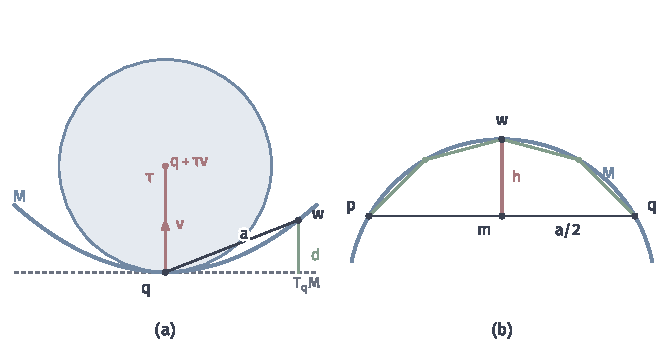
\includegraphics[width=112mm]{figures/04-spaces-measures-and-geometry/04-manifolds/matplotlib/mrec-rolling-ball/figure.pdf}
  \caption{可达半径的两个局部结论。(a) 半径为$\tau$的球（浅蓝）贴在$M$上，内部不含$M$的点，由此$\bm w$到切线的距离$d\leq a^2/(2\tau)$，其中$a$是$\bm q$到$\bm w$的弦长。(b) 半径为$\tau$的圆是引理~\ref{lem:mrec-midpoint}的极端情形：弦$\bm p\bm q$的中点$\bm m$投影到$\bm w$，两段新弦（绿）的长度恰为$2\tau\sin(\theta/2)$；继续细分，折线长度趋于弧长$2\tau\theta$。}
  \label{fig:mrec-rolling-ball}
\end{BookInlineFigure}

要控制沿流形的路程，办法是不断取弦的中点并投影回$M$，每投影一次，弦就更贴近流形，如图~\ref{fig:mrec-rolling-ball}(b)。下面的引理把一次投影的效果算清楚：它对中点的最近点用两次式~\eqref{eq:mrec-reach-normal}，把$\bm p$、$\bm q$到它的距离一起控制住。

\begin{lemma}[中点投影]
\label{lem:mrec-midpoint}
设$\bm p,\bm q\in M$，$a=\lVert\bm p-\bm q\rVert_2<2\tau$，把$a$写成$2\tau\sin\theta$，$\theta\in[0,\pi/2)$。则存在$\bm w\in M$，使
\begin{equation}
 \max\bigl(\lVert\bm p-\bm w\rVert_2,\ \lVert\bm q-\bm w\rVert_2\bigr)\leq2\tau\sin\frac\theta2 .
 \label{eq:mrec-midpoint}
\end{equation}
\end{lemma}
\begin{proof}
令$\bm m=\tfrac12(\bm p+\bm q)$，它到$\bm p$的距离是$a/2$，所以$\operatorname{dist}(\bm m,M)\leq a/2<\tau$，可取最近点$\bm w=\pi(\bm m)$，记$h=\lVert\bm m-\bm w\rVert_2$。

$h=0$时$\bm w=\bm m$，到两端的距离都是$a/2$，而
\[
 \frac a2=\tau\sin\theta\leq2\tau\sin\frac\theta2 ,
\]
结论成立。下设$h>0$。

令$\bm v=(\bm m-\bm w)/h$，由一阶条件，$\bm v$是$\bm w$处的单位法向量。记$c=\langle\bm p-\bm m,\bm v\rangle$，由对称性不妨设$c\geq0$，再记$A=a^2/4+h^2$。

按$\bm p-\bm w=(\bm p-\bm m)+(\bm m-\bm w)$展开，并用$\bm q-\bm m=-(\bm p-\bm m)$，得
\[
 \lVert\bm p-\bm w\rVert_2^2=A+2hc,\qquad\lVert\bm q-\bm w\rVert_2^2=A-2hc .
\]
同时，$\bm p-\bm w$在$\bm v$上的分量是$h+c$，$\bm q-\bm w$在$\bm v$上的分量是$h-c$。

对$\bm p$、$\bm w$与$\bm q$、$\bm w$分别用式~\eqref{eq:mrec-reach-normal}，得
\[
 h+c\leq\frac{A+2hc}{2\tau},\qquad h-c\leq\frac{A-2hc}{2\tau}.
\]
两式相加，得到
\[
 2\tau h\leq A,\qquad\text{即}\quad h^2-2\tau h+\frac{a^2}4\geq0 .
\]
又$h\leq a/2<\tau$，所以$h$不超过这个二次式的较小根：
\[
 h\leq h_*=\tau-\sqrt{\tau^2-a^2/4}=\tau(1-\cos\theta).
\]

从第一式解出$c$，由$\tau-h>0$，
\[
 c\leq\frac{A-2\tau h}{2(\tau-h)}.
\]
代回$\lVert\bm p-\bm w\rVert_2^2=A+2hc$，整理得
\[
 \lVert\bm p-\bm w\rVert_2^2\leq g(h)=\frac{\tau(a^2/4-h^2)}{\tau-h}.
\]

对$g$求导，
\[
 g'(h)=\frac{\tau(h^2-2\tau h+a^2/4)}{(\tau-h)^2}\geq0,\qquad 0\leq h\leq h_*,
\]
所以$g(h)\leq g(h_*)$。用$a/2=\tau\sin\theta$代入，
\[
 g(h_*)=\frac{\tau\cdot2\tau^2\cos\theta(1-\cos\theta)}{\tau\cos\theta}=2\tau^2(1-\cos\theta)=\bigl(2\tau\sin\tfrac\theta2\bigr)^2 .
\]
由$c\geq0$，$\bm q$到$\bm w$的距离不超过$\bm p$到$\bm w$的距离，所以两段距离都不超过$2\tau\sin(\theta/2)$。
\end{proof}

把式~\eqref{eq:mrec-reach-normal}和反复投影的结果写在一起，就是后面各节反复使用的两条局部推论。

\begin{theorem}[可达半径的局部推论]
\label{thm:mrec-reach-consequences}
设$M$的可达半径为$\tau>0$，$\bm p,\bm q\in M$。则$\bm q-\bm p$到$T_{\bm p}M$的距离满足式~\eqref{eq:mrec-reach-normal}。若$\lVert\bm p-\bm q\rVert_2<2\tau$，则$\bm p,\bm q$属于同一分支，并且
\begin{equation}
 d_M(\bm p,\bm q)\leq2\tau\arcsin\frac{\lVert\bm p-\bm q\rVert_2}{2\tau}.
 \label{eq:mrec-reach-arc}
\end{equation}
\end{theorem}

\begin{proof}
第一条就是引理~\ref{lem:mrec-normal-distance}。再看第二条，由引理~\ref{lem:mrec-component-gap}，$\bm p,\bm q$在同一分支。把$\lVert\bm p-\bm q\rVert_2$写成$2\tau\sin\theta$，$\theta<\pi/2$。对$\bm p,\bm q$用引理~\ref{lem:mrec-midpoint}得到$\bm w$，再对$(\bm p,\bm w)$和$(\bm w,\bm q)$分别用一次，如此重复$k$轮。

每轮把相邻两点弦长对应的角减半，$k$轮后得到$M$上$2^k+1$个点，相邻点的距离都不超过$2\tau\sin(\theta/2^k)$，这些弦长的总和不超过
\[
 2^k\cdot2\tau\sin\frac\theta{2^k}\leq2\tau\theta .
\]
在紧致流形上，$\lVert\bm x-\bm y\rVert_2\to0$时$d_M(\bm x,\bm y)/\lVert\bm x-\bm y\rVert_2$一致趋于$1$，因为$M$在小尺度上是斜率很小的图。所以对任意$\eta>0$，$k$足够大时
\[
 d_M(\bm p,\bm q)\leq(1+\eta)\,2\tau\theta .
\]
令$\eta\to0$，并由$\theta=\arcsin(\lVert\bm p-\bm q\rVert_2/2\tau)$，得式~\eqref{eq:mrec-reach-arc}。
\end{proof}

两条结论在圆上都取等号。在半径为$R$的圆上，取$\bm p$处的切线为水平方向，$\bm q$对应圆心角$\theta$，则法向分量为$R(1-\cos\theta)$，弦长的平方为$2R^2(1-\cos\theta)$，式~\eqref{eq:mrec-reach-normal}取等号；弦长$s$对应的弧长为$2R\arcsin(s/2R)$，式~\eqref{eq:mrec-reach-arc}也取等号。所以这两个估计不能再改进。

第一条说，在半径为$r$的邻域内，流形偏离切平面至多$r^2/(2\tau)$，相对于邻域半径的比值是$r/(2\tau)$。第二条说，环境距离小于$2\tau$的两点，沿流形的距离不会比直线长太多：$\lVert\bm p-\bm q\rVert_2\leq\tau$时，比值至多为$2\arcsin\tfrac12=\pi/3\approx1.047$。

第一条还给出弯曲的上界。设$\gamma$是$M$上过$\bm p$的单位速度测地线，$\gamma(s)-\bm p$的切向部分近似$s\gamma'(0)$，法向部分近似$\tfrac12s^2\gamma''(0)$，而弦长近似$s$。代入式~\eqref{eq:mrec-reach-normal}，令$s\to0$，得$\lVert\gamma''(0)\rVert_2\leq1/\tau$，即每条测地线作为$\mathbb R^D$中的曲线，曲率都不超过$1/\tau$。

\subsection{邻域尺度}
\label{sec:mrec-neighborhood-scale}

局部计算的成败，关键在邻域半径$r$的选取。图~\ref{fig:mrec-scale}用同一组带噪声的样本比较了三种半径。

$r$过小时，邻域内的样本太少，甚至只有中心自己。即使样本不少，若$r$与扰动界$\sigma$同量级，邻域内样本的散布主要来自噪声，看不出流形的方向，如图(a)。所以$r$要明显大于覆盖精度$\delta_P$和$\sigma$。

$r$过大时出现另外两类问题。由定理~\ref{thm:mrec-reach-consequences}，流形在邻域内偏离切平面可达$r^2/(2\tau)$，$r$与$\tau$可比时这一偏离与邻域本身一样大，局部已不能看成平的。另外，$r$超过两股的间隔时，邻域会同时包含两股的样本，如图(c)，它们在环境中靠近，沿流形却相距很远。

由定理~\ref{thm:mrec-reach-consequences}的第二条，$r<2\tau$时邻域内的点都属于同一分支；要使局部线性近似可靠，还要$r$远小于$\tau$。所以分析的范围大致是
\begin{equation}
 \delta_P,\ \sigma\ll r\ll\tau .
 \label{eq:mrec-scale-range}
\end{equation}

\begin{BookInlineFigure}
  \centering
  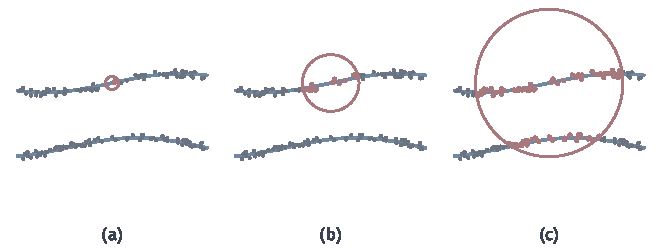
\includegraphics[width=112mm]{figures/04-spaces-measures-and-geometry/04-manifolds/matplotlib/mrec-scale/figure.pdf}
  \caption{同一组带噪声的样本在三种邻域半径下的情形，两条蓝线是流形的两股，红点是邻域内的样本。(a) 半径与噪声同量级，邻域内只有零星几个点。(b) 半径适中，邻域内的样本沿一股展开。(c) 半径超过两股的间隔，邻域混入另一股的样本。}
  \label{fig:mrec-scale}
\end{BookInlineFigure}

\paragraph{嵌入弯曲决定局部线性误差}

第~\ref{chap:riemannian-geometry}章区分了内在曲率与嵌入弯曲。半径为$\rho$的圆柱面内在地是平的，可以展开成平面而不改变任何长度，如图~\ref{fig:mrec-cylinder}(b)；但它在$\mathbb R^3$中弯曲，可达半径为$\rho$，切平面只在一条母线上贴着它，如图~\ref{fig:mrec-cylinder}(a)。

取$\rho=1$，沿圆周方向取一点，弦长$r=0.5$，它对应的圆心角$\theta$满足$2\sin(\theta/2)=0.5$，到切平面的距离是
\[
 1-\cos\theta=\frac{r^2}{2\rho}=0.125 .
\]
内在曲率为零并没有让这一偏离消失；沿母线方向偏离却恰好是零。这说明局部线性误差首先由环境中的嵌入形状决定，可达半径度量的正是这一形状，内在曲率是另一回事。

\begin{BookInlineFigure}
  \centering
  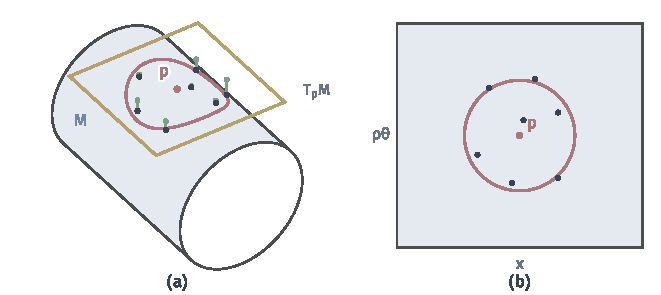
\includegraphics[width=112mm]{figures/04-spaces-measures-and-geometry/04-manifolds/matplotlib/mrec-cylinder/figure.pdf}
  \caption{圆柱面的内在几何与嵌入形状。(a) 点$\bm{p}$处的切平面（黄色框）与红圈内的邻域，绿色线段是样本（黑点）到切平面的法向偏离，沿圆周方向偏离最大。(b) 把圆柱面沿母线剪开摊平，同一邻域和样本成为平面上的圆盘和点，长度不变，内在曲率为零。}
  \label{fig:mrec-cylinder}
\end{BookInlineFigure}

反过来，即使嵌入弯曲很小，邻域内样本的方向覆盖仍需单独核验，第~\ref{sec:mrec-coverage}节的水平线采样就是例子。选定$r$以后，邻域应同时满足三条：足够小，使弯曲可以忽略；足够大，使样本数和散布压过噪声；样本在各个切向上都有展开。
